%JULIA HEADER
\documentclass{article}
\usepackage{amsmath,amsthm}
\usepackage{amssymb,latexsym}
\usepackage{epsfig}
\usepackage{hyperref}
\usepackage{float}
\usepackage{fullpage}
\usepackage{enumerate}
\usepackage{paralist}
\usepackage{times}
\usepackage{tikz}
\usetikzlibrary{automata, positioning}


\newtheorem{theorem}{Theorem}
\newtheorem{corollary}[theorem]{Corollary}
\newtheorem{question}[theorem]{Question}
\newtheorem{lemma}[theorem]{Lemma}
\newtheorem{observation}[theorem]{Observation}
\newtheorem{proposition}{Proposition}
\newtheorem{definition}[theorem]{Definition}
\newtheorem{claim}[theorem]{Claim}
\newtheorem{fact}[theorem]{Fact}
\newtheorem{assumption}[theorem]{Assumption}
\newtheorem{example}{Example}
\newtheorem{conjecture}[theorem]{Conjecture}
\newtheorem{alg}[theorem]{Algorithm}

\newcommand{\myparagraph}[1]{\paragraph{#1.}}

\newcommand{\eps}{\varepsilon}
\newcommand{\epssdp}{\varepsilon_{\rm sdp}}

\newcommand{\C}{C}
\newcommand{\Tr}{Tr} %CHECK
\newcommand{\Id}{Id} %CHECK
\newcommand{\Exs}[2]{E_{#1}[#2]} %CHECK

\newcommand{\trace}{{\rm Tr}}

\newcommand{\norm}[1]{\left\|\,#1\,\right\|}       % norm
\newcommand{\onorm}[1]{\norm{#1}_{\mathrm{1}}}      % Euclidean norm for vectors
\newcommand{\enorm}[1]{\norm{#1}_{\mathrm{2}}}      % Euclidean norm for vectors
\newcommand{\trnorm}[1]{\norm{#1}_{\mathrm {tr}}}  % trace norm
\newcommand{\fnorm}[1]{\norm{#1}_{\mathrm {F}}}    % frobenius norm
\newcommand{\snorm}[1]{\norm{#1}_{\mathrm {\infty}}}    % spectral norm

\newcommand{\set}[1]{{\left\{#1\right\}}}    % braces for set notation
\newcommand{\ve}[1]{\mathbf{#1}}
\newcommand{\abs}[1]{\left\lvert #1 \right\rvert}

\newcommand{\complex}{{\mathbb C}}
\newcommand{\reals}{{\mathbb R}}
\newcommand{\ints}{{\mathbb Z}}
\newcommand{\nats}{{\mathbb N}}

\newcommand{\proj}[1]{\mbox{$|#1\rangle \!\langle #1 |$}}
\newcommand{\enc}[1]{\left<#1\right>}

\newcommand{\spa}[1]{\mathcal{#1}}
\newcommand{\dens}{D(\spa{A}\otimes\spa{B})}
\newcommand{\unitaries}{U(\spa{A}\otimes\spa{B})}

\bibliographystyle{alpha}

\begin{document}

\title{CMSC 303 Introduction to Theory of Computing, VCU\\Spring 2017, Assignment 3\\Due: Thursday, February 23, 2017\\Matthew Bowers}
\date{}
\maketitle
\noindent Worked with Samuel Yound and Sean McDermott
\noindent Total marks: $66$ marks $+$ $4$ marks bonus $+$ $8$ bonus marks for LaTeX\\

\noindent Unless otherwise noted, the alphabet for all questions below is assumed to be $\Sigma=\set{0,1}$.
%\section{Questions}
\begin{enumerate}
    \item {[12 marks]} This question develops your ability to devise regular expressions, given an explicit definition of a language. For each of the following languages, prove they are regular by giving a regular expression which describes them. Justify your answers.
        \begin{enumerate}
            \item $L=\set{x\mid x \text{ begins with a $0$ and ends with a $1$}}$.\\
            \\
            $0\Sigma^*1$\\
            \item $L=\set{x\mid x \text{ contains at least four $0$'s}}$\\
            \\
            $\Sigma^*0\Sigma^*0\Sigma^*0\Sigma^*0\Sigma^*$\\
            \item $L=\set{1, 11, \epsilon}$.\\
            \\
            $1\cup11\cup\epsilon$\\
            \item $L=\set{x\mid \text{the length of $x$ is at most $3$}}$.\\
            \\
            $\epsilon \cup \Sigma \cup \Sigma\Sigma \cup \Sigma\Sigma\Sigma$\\
            \item $L=\set{x\mid x \text{ doesn't contain the substring $110$}}$.\\
            \\
            $0^* \cup 1^* \cup (0^*100^*)^*1^* \cup (0^*1^*)$
            \item $L=\set{x \mid \abs{x}>0 \text{, i.e. $x$ is non-empty}}$.\\
            \\
            $\Sigma\Sigma^*$\\
        \end{enumerate}
    \item {[20 marks]} This question tests your understanding of how to translate a regular expression into a finite automaton. Using the construction of Lemma 1.55, construct NFAs recognizing the languages described by the following regular expressions.
        \begin{enumerate}
            \item {[5 marks]} $R=\emptyset^*$.\\
            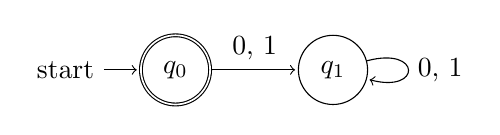
\begin{tikzpicture}[shorten >=1pt,node distance=2cm,on grid,auto] 
		\node[state,initial, accepting] (q_0)   {$q_0$}; 
		\node[state] (q_1) [right=of q_0] {$q_1$};
		\path[->]
			(q_0) edge  node {0, 1} (q_1)
			(q_1) edge [loop right] node {0, 1} ();
   	\end{tikzpicture}
            \item {[15 marks]} $R=(0\cup 1)^*111(0\cup 1)^*$.\\
            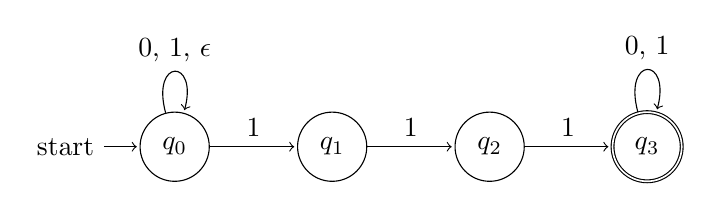
\begin{tikzpicture}[shorten >=1pt,node distance=2cm,on grid,auto] 
		\node[state,initial] (q_0)   {$q_0$}; 
		\node[state] (q_1) [right=of q_0] {$q_1$};
		\node[state] (q_2) [right=of q_1] {$q_2$};
		\node[state, accepting] (q_3) [right=of q_2] {$q_3$};
		\path[->]
			(q_0) edge [loop above] node {0, 1, $\epsilon$} ()
			(q_0) edge node {1} (q_1)
			(q_1) edge node {1} (q_2)
			(q_2) edge node {1} (q_3)
			(q_3) edge [loop above] node {0, 1} ();
   	\end{tikzpicture}
        \end{enumerate}
    \item {[15 marks]} This question tests your understanding of how to translate a finite automaton into a regular expression. Consider DFA $M=(Q,\Sigma,\delta,q,F)$ such that $Q=\set{q_1,q_2,q_3}$, $q=q_1$, $F=\set{q_1,q_3}$, and $\delta$ is given by:
                \[
\begin{tabular}{|c|cc|}
  \hline
  $\delta$ & 0 & 1 \\
  \hline
  $q_1$ & $q_2$ & $q_2$\\
  $q_2$ & $q_2$ & $q_3$\\
  $q_3$ & $q_1$ & $q_2$\\
  \hline
\end{tabular}
        \]
            Draw the state diagram for $M$, and then apply the construction of Lemma 1.60 to obtain a regular expression describing $L(M)$.\\
            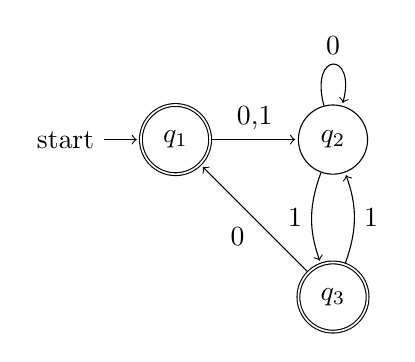
\begin{tikzpicture}[shorten >=1pt,node distance=2cm,on grid, auto]
            \node [state, initial, accepting] (q_1) {$q_1$};
            \node [state] [right =of q_1] (q_2) {$q_2$};
            \node [state, accepting] [below =of q_2] (q_3) {$q_3$};
            \path[->]
            	(q_1) edge node {0,1} (q_2)
            	(q_2) edge [bend right=20] node [swap] {1} (q_3)
            	(q_2) edge [loop above] node {0} ()
            	(q_3) edge node {0} (q_1)
            	(q_3) edge [bend right= 20] node [swap] {1} (q_2);
            \end{tikzpicture}
\\
\newpage
Transform into a GNFA.\\
	Step 1.
            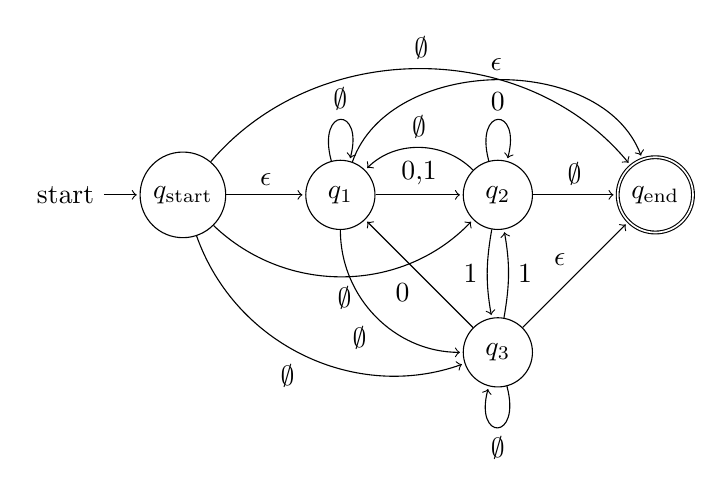
\begin{tikzpicture}[shorten >=1pt,node distance=2cm,on grid, auto]
            \node [state, initial] (q_s) {$q_{\text{start}}$};
            \node [state] [right=of q_s] (q_1) {$q_1$};
            \node [state] [right =of q_1] (q_2) {$q_2$};
            \node [state] [below =of q_2] (q_3) {$q_3$};
            \node [state, accepting] [right=of q_2] (q_e) {$q_{\text{end}}$};
            \path[->]
            	(q_s) edge node {$\epsilon$} (q_1)
            		edge [bend right=45] node [swap] {$\emptyset$} (q_2)
            		edge [bend right=45] node [swap] {$\emptyset$} (q_3)
            		edge [bend left=50] node {$\emptyset$} (q_e)
            	(q_1) edge node {0,1} (q_2)
            		edge [bend left= 70] node {$\epsilon$} (q_e)
            		edge [loop above] node {$\emptyset$} ()
            		edge [bend right=45] node [swap] {$\emptyset$} (q_3)
            	(q_2) edge [bend right=10] node [swap] {1} (q_3)
            		edge [bend right =45] node [swap] {$\emptyset$} (q_1)
            		edge node {$\emptyset$} (q_e)
            	(q_2) edge [loop above] node {0} ()
            	(q_3) edge node {0} (q_1)
            	(q_3) edge [bend right= 10] node [swap] {1} (q_2)
            		edge [loop below] node {$\emptyset$} ()
            		edge node {$\epsilon$} (q_e);
            \end{tikzpicture}
	\\ Step 2
            \begin{tikzpicture}[shorten >=1pt,node distance=4cm,on grid, auto]
            \node [state, initial] (q_s) {$q_{\text{start}}$};
            \node [state] [right =of q_s] (q_2) {$q_2$};
            \node [state] [below =of q_2] (q_3) {$q_3$};
            \node [state, accepting] [right=of q_2] (q_e) {$q_{\text{end}}$};
            \path[->]
            	(q_s) edge node {$0\cup1$} (q_2)
            		edge [bend left=65] node {$\epsilon$} (q_e)
            		edge node [swap] {$\emptyset$} (q_3)
            	(q_2) edge [bend right=30] node [swap] {1} (q_3)
            		edge node {$\emptyset$} (q_e)
            		edge [loop above] node {0} ()
            	(q_3) edge node [sloped, anchor=center, above] {$0\Sigma\cup1$} (q_2)
            		edge [loop below] node {$\emptyset$} ()
            		edge node {$0\cup\epsilon$} (q_e);
            \end{tikzpicture}
	\\ Step 3
            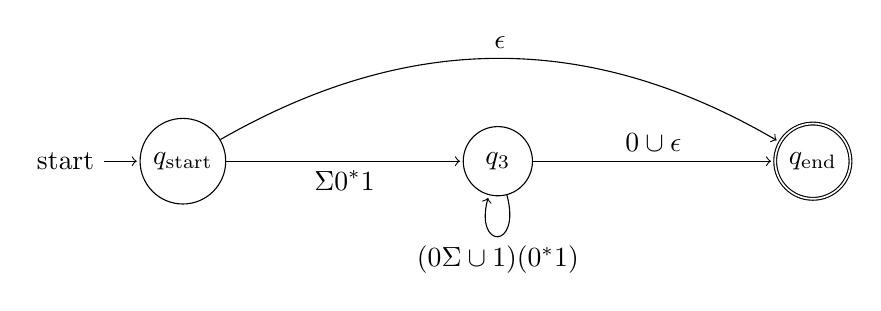
\begin{tikzpicture}[shorten >=1pt,node distance=4cm,on grid, auto]
            \node [state, initial] (q_s) {$q_{\text{start}}$};
            \node [state] [right =of q_s] (q_3) {$q_3$};
            \node [state, accepting] [right=of q_3] (q_e) {$q_{\text{end}}$};
            \path[->]
            	(q_s) edge [bend left] node {$\epsilon$} (q_e)
            		edge node [swap] {$\Sigma0^*1$} (q_3)
            	(q_3) edge [loop below] node {$(0\Sigma\cup1)(0^*1)$} ()
            		edge node {$0\cup\epsilon$} (q_e);
            \end{tikzpicture}
	\\ Step 4
            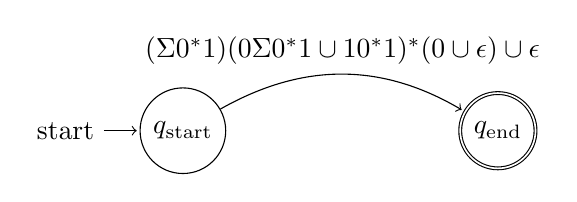
\begin{tikzpicture}[shorten >=1pt,node distance=4cm,on grid, auto]
            \node [state, initial] (q_s) {$q_{\text{start}}$};
            \node [state, accepting] [right=of q_s] (q_e) {$q_{\text{end}}$};
            \path[->]
            	(q_s) edge [bend left] node {$(\Sigma0^*1)(0\Sigma0^*1\cup10^*1)^*(0\cup\epsilon)\cup\epsilon$} (q_e); 		
            \end{tikzpicture}
    \item {[15 marks]} This question allows you to practice proving a language is non-regular via the Pumping Lemma. Using the Pumping Lemma (Theorem 1.70), give formal proofs that the following languages are \emph{not} regular:
        \begin{enumerate}
            \item $L=\set{www\mid w\in\set{0,1}^*}$.\\
            \begin{proof}
            For a proof by contradiction assume L is a regular language.\\
            This implies that $\exists$ a pumping length p.\\
            Choose $s = 0^p10^p10^p1$\\
            $s \in B$ and $|s| \geq p$\\
            By pumping lemma $\exists x, y, z$ s.t. $s=xyz$ and 
            $|xy|\leq p \implies x, y$ contains only 0's\\
            $|p| > 0$\\
            $xy^0z = 0^{p'}10^p10^p1$ where $p' < p \implies xy^0z \notin B \bot \therefore B$ is not regular.             
            \end{proof}
            \item $L=\set{1^n0^m1^n\mid m\text{, }n\geq 0}$.
            \begin{proof}
            For a proof by contradiction assume L is a regular language.\\
            This implies that $\exists$ a pumping length p.\\
            Choose $s =1^p0^m1^p$\\
            $s\in L$\\
            $|s|=2p+m \geq p$\\
            The conditions for the pumping are met\\
            $\exists x, y, z$ s.t. $s=xyz$ and $|xy|\leq p \therefore$ every character in x and y is a 1 and y 
            contains at least one 1.
            $xy^2z = 1^(p')0^m1^p$ where $p'\geq p \therefore xy^2z \notin L$ This is a contradiction. 
            \end{proof}
            \item $L=\set{x\mid x\in\set{0,1}^*\text{ is not a palindrome}}$. Recall a palindrome is a string that looks the same forwards and backwards. Examples of palindromes are ``madam'' and ``racecar''.\\
            \begin{proof}
            For a proof by contradiction assume L is a regular language. Because RL's are closed under compliment $\neg L$ is also a regular language. The negation of L is that x is a palindrome.\\
            This implies that $\exists$ a pumping length p.\\
            Choose $s = 1^p01^p$\\
            $s \in \neg L$ and $|s| \geq p$ meets the conditions of the pumping lemma so\\
            $\exists x, y, z$ s.t. $s =xyz$ and $|xy| \leq p \implies$ every character in x and y is a 1. \\
            consider $xy^2z = 1^{p'}01^p$ $p' > p \therefore xy^2z \notin L$ this is a controdiction to the implication that 
            $\neg L$ is a regular language, so our assumption that L was a regular language must be incorrect.
            \end{proof}
        \end{enumerate}
    \item  {[$4$ marks $+$ $4$ marks bonus]} This question reveals important subtleties of the Pumping Lemma. Let $B=\set{0^kx0^k \mid k\geq 1\text{ and } x\in\Sigma^*}$.
                \begin{enumerate}
                \item{[4 marks]} Consider the following argument, which claims to prove that $B$ is not regular.

                    Assume $B_2$ is regular, and let $p$ be the pumping length. Consider string $s=0^p10^p\in B_2$, and decompose it as $s=xyz$ with $x=\epsilon$, $y=0^p$, $z=10^p$. Then, pumping $s$ down by setting $i=0$ yields string $s'=xy^iz=xy^0z=10^p\not \in B_2$. Hence, by the Pumping Lemma, we have a contradiction. We conclude that $B_2$ is not regular.

                 	The question is: What is wrong with this proof?\\
                    \\
                    The pumping lemma states that some x, y, z must exist. This proof has shown that this particular choice of x, y, and z does not work, but it does not prove that there is no possible choice.
                \item {[4 marks, bonus]} Prove that, in fact, $B$ is regular.\\
                This language can be expressed as $0\Sigma^*0$ Because x can be any number of any character extra zeros before or after can be absorbed into the sigma. 
            \end{enumerate}
\end{enumerate}
\end{document}
